\documentclass[11pt,aspectratio=169,dvipsnames]{beamer}
\graphicspath{{figs/}}
\usetheme{default}
\usepackage{DasBeamerPaket}
\usepackage{animate}
\usepackage{lastpage}
\usepackage{appendixnumberbeamer}
\usepackage{braket}
\usepackage{tikz}
\setbeamercolor{section in toc}{fg=NavyBlue}
\setbeamercolor{frametitle}{fg=NavyBlue}
\captionsetup[figure]{labelfont=bf}
\captionsetup[table]{labelfont=bf}
\newcommand{\theauthor}{Jakob Krause}
\newcommand{\theshortauthor}{\textsc{J. Krause} for CBELSA/TAPS}
\newcommand{\authormail}{krause@hiskp.uni-bonn.de}
\newcommand{\authorgit}{krausejm}
\newcommand{\thetitle}{Recent Polarization Observable Results in  $\eta$- and $\eta'$-photoproduction off the proton}
\newcommand{\theshorttitle}{$\Sigma$ in $\eta$- and $\eta'$ photoproduction}
\newcommand{\thecolor}{black!70!blue}
\newcommand{\thecolorr}{black!60!blue}
\newcommand{\thecolorrr}{black!50!blue}
\newcommand{\thesubtitle}{Master thesis for the CBELSA/TAPS collaboration}
\newcommand{\thedate}{30th March 2022}
\makeatletter
\patchcmd{\beamer@calculateheadfoot}{\advance\footheight by 4pt}{\advance\footheight by 20pt}{}{}
\makeatother
\begin{document}
	\definecolor{myWhite}{rgb}{1,1,1}
	
	
	\setbeamercolor{coloredboxstuff}{fg=myWhite,bg=\thecolor}
	\setbeamercolor{coloredboxstuff1}{fg=myWhite,bg=\thecolorr}
	\setbeamercolor{coloredboxstuff2}{fg=myWhite,bg=\thecolorrr}	
	\makeatother
	\setbeamertemplate{footline}
	{
		\leavevmode%
		\hbox{%
			\begin{beamercolorbox}[wd=.33\paperwidth,ht=2.25ex,dp=1ex,center]{coloredboxstuff}%
				{\theshortauthor}
			\end{beamercolorbox}%
			\begin{beamercolorbox}[wd=.34\paperwidth,ht=2.25ex,dp=1ex,center]{coloredboxstuff}%
				{\theshorttitle}
			\end{beamercolorbox}%
			\begin{beamercolorbox}[wd=.33\paperwidth,ht=2.25ex,dp=1ex,center]{coloredboxstuff}%
				\insertframenumber{} / \inserttotalframenumber\hspace*{1ex}
		\end{beamercolorbox}}%
	}
	\makeatletter
	
	
	\setbeamercovered{transparent}
	\setbeamertemplate{navigation symbols}{}
	\setbeamertemplate{frametitle}[default][left,leftskip=0.5cm]
	\setbeamertemplate{itemize item}{\color{black}$\blacktriangleright$}
	\setbeamertemplate{section in toc}[sections numbered]
	\setbeamercolor{section in toc}{fg=\thecolor}
	\setbeamercolor{frametitle}{fg=\thecolor}
	\captionsetup{font=scriptsize,labelfont=scriptsize}
	\AtBeginSection[]
	{	
		
		{
			
			\makeatother
			\setbeamertemplate{footline}
			{
				\leavevmode%
				\hbox{%
					\begin{beamercolorbox}[wd=.34\paperwidth,ht=2.25ex,dp=1ex,center]{coloredboxstuff}%
						{|\hfill\theshortauthor\hfill|}
					\end{beamercolorbox}%
					\begin{beamercolorbox}[wd=.34\paperwidth,ht=2.25ex,dp=1ex,center]{coloredboxstuff}%
						{\theshorttitle}
					\end{beamercolorbox}%
					\begin{beamercolorbox}[wd=.34\paperwidth,ht=2.25ex,dp=1ex,center]{coloredboxstuff}%
						\insertsection\hspace*{1ex}
				\end{beamercolorbox}}%
			}
			\makeatletter
			
			
			\begin{frame}[noframenumbering]
				\frametitle{}
				\addtocounter{page}{-1}
				\tableofcontents[currentsection]
			\end{frame}
		}
		
	}
	%\begin{frame}[plain]
	%	\centering
	%	{\Large \color{\thecolor}{\thetitle}}\\
	%	\vspace{0.5cm}
	%	{\thesubtitle}
	%	\vfill
	%	\begin{minipage}{\linewidth}
	%		\centering
	%		\begin{minipage}{\linewidth}
	%			\textsc{\theauthor}\\
	%			\scriptsize \href{mailto:\authormail}{\faEnvelope  \hspace*{0.1cm}\authormail} {\color{black}$|$} \href{https://github.com/\authorgit}{\faGithub  \hspace*{0.1cm}\authorgit}\\
	%		\end{minipage}
	%		\vspace{.5cm}
			
	%		{\scriptsize
	%			Supervisor: \textsc{Jun. Prof. Dr. Annika Thiel}\\
	%			\tiny \href{mailto:thiel@hiskp.uni-bonn.de}{\faEnvelope  \hspace*{0.1cm}thiel@hiskp.uni-bonn.de}\par}
	%	\end{minipage}
	%	\vspace{0.2cm}
		
	%	\thedate
	%\end{frame}
	
\begin{frame}{Event based maximum likelihood fit}
	\begin{align*}
		-\ln\mathcal{L}=&\sum_{i=1}^{n}-\ln(p_\text{prompt}(\phi_i,p_{\gamma,i},\Sigma,a_1\dots a_4,b_1\dots b_4))+\\
		&\sum_{j=1}^{m}-\ln\left(p_\text{sideband}(\phi_j,p_{\gamma,j},\Sigma^\text{bkg},a_1^\text{bkg}\dots a_4^\text{bkg},b_1^\text{bkg}\dots b_4^\text{bkg})\right)
	\end{align*}
where
\begin{align*}
	p_\text{prompt}&=f_{\text{sig}}\cdot\tilde{p}(\phi,p_\gamma,\Sigma,a_1\dots a_4, b_1\dots b_4)\\ &+ \left(1-f_\text{sig}\right)\cdot\tilde{p}(\phi,p_\gamma,\Sigma^\text{bkg},a_1^\text{bkg}\dots a_4^\text{bkg}, b_1^\text{bkg}\dots b_4^\text{bkg})\\
	p_\text{sideband}&=\tilde{p}(\phi,p_\gamma,\Sigma^\text{bkg},a_1^\text{bkg}\dots a_4^\text{bkg}, b_1^\text{bkg}\dots b_4^\text{bkg})
\end{align*}
and \begin{equation*}
	\tilde{p}(\phi,\Sigma)=\frac{\left(1+p_\gamma\Sigma\cos\left(2\left(\alpha^\parallel-\phi\right)\right)\right)\cdot\left(\sum_{k=0}^{4}a_k\sin(k\phi)+b_k\cos(k\phi)\right)}{1-\frac{1}{2}a_2p_\gamma\Sigma}
\end{equation*}
\end{frame}
\begin{frame}{Event based maximum likelihood fit (in STAN)}
define priors and implement log-likelihood, truncate $\Sigma$ to $[-1,1]$
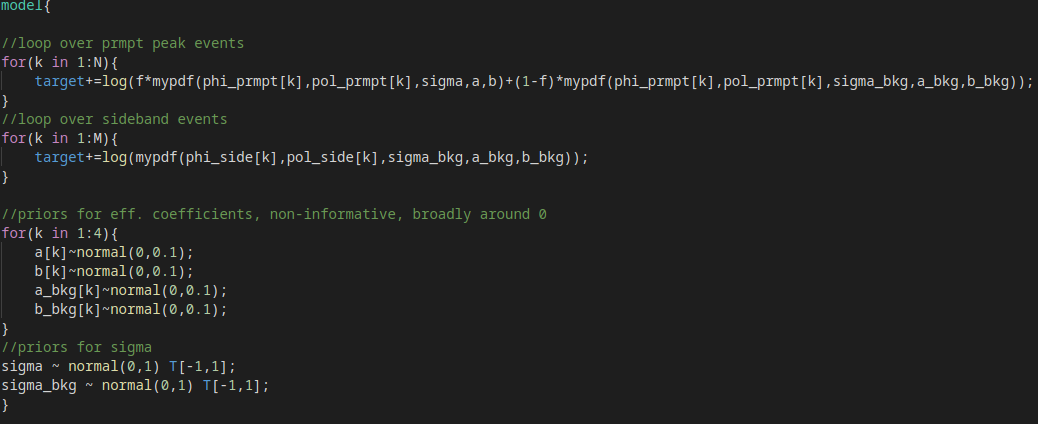
\includegraphics[width=\linewidth]{stan_snippet.png}	
	
\end{frame}
\begin{frame}{Fit diagnostics}
	4 chains, 5000 samples, 1000 sample warmup
	\begin{itemize}


	\item ppd checks not possible (similar to "normal" event-based ML fit) $\to$ toy MC (?)
	
	\item$\hat{R}=1$ for all parameters and all fits
	
	\item MCSE of median small: (nsamples chosen s.t. rel. error $\lesssim0.05$)\\ 
	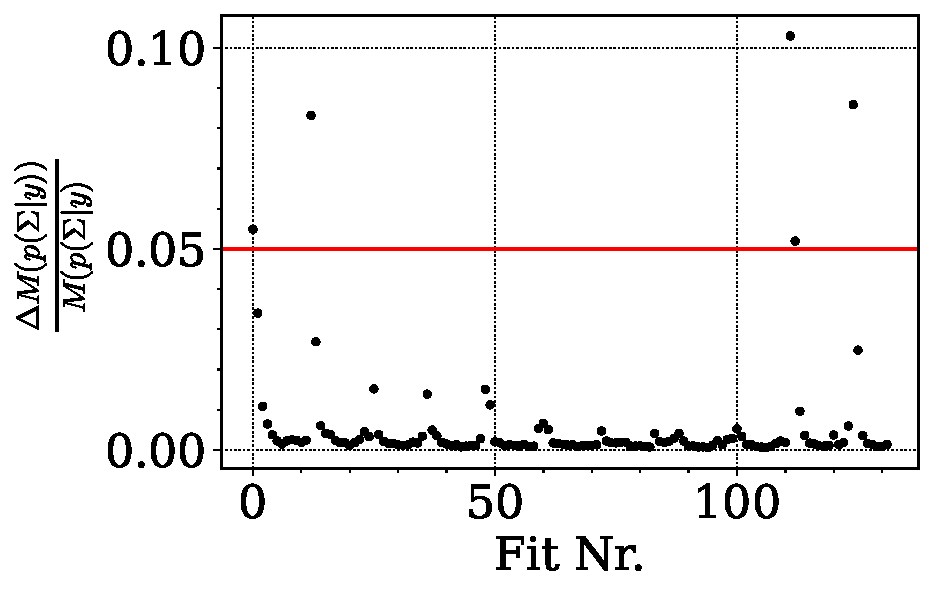
\includegraphics[width=.5\linewidth]{../../bayes/event_based_fit/mcse.pdf}
	\item check efficiency function (?)
	\end{itemize}
\end{frame}
\begin{frame}{Results}
	\centering
	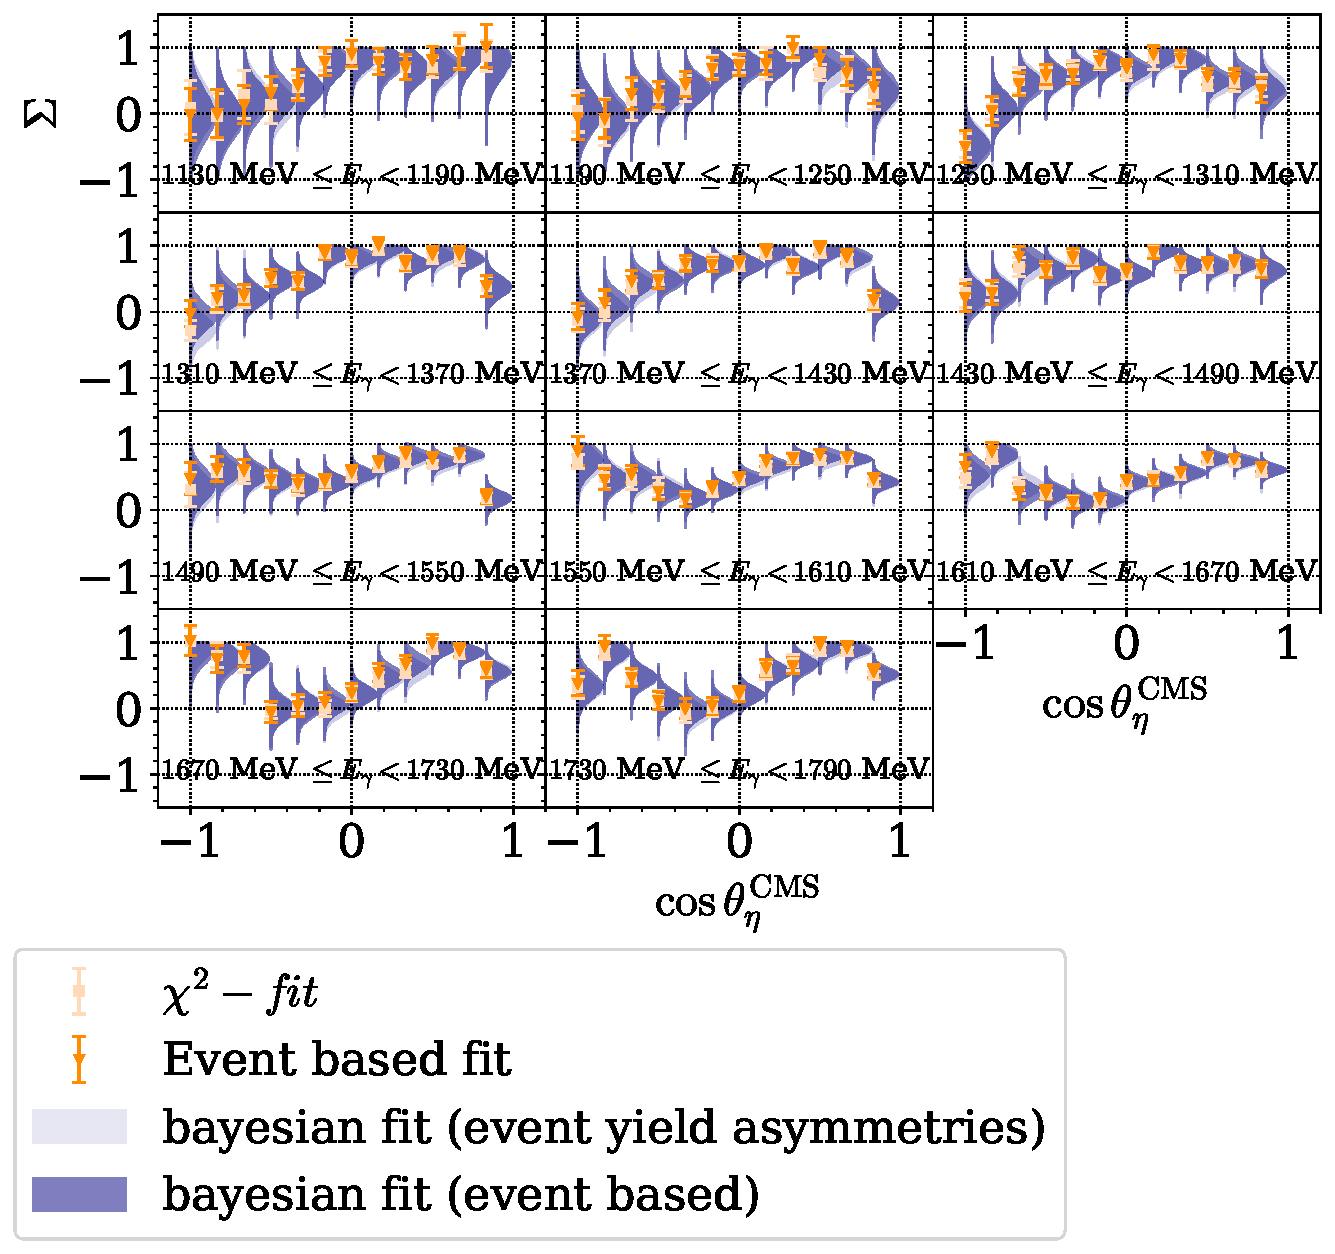
\includegraphics[width=.6\linewidth]{../../bayes/event_based_fit/sigma_eta_alt.pdf}
\end{frame}


\begin{frame}{$\Sigma$ in $\gamma p \to p 2\pi^0$}
	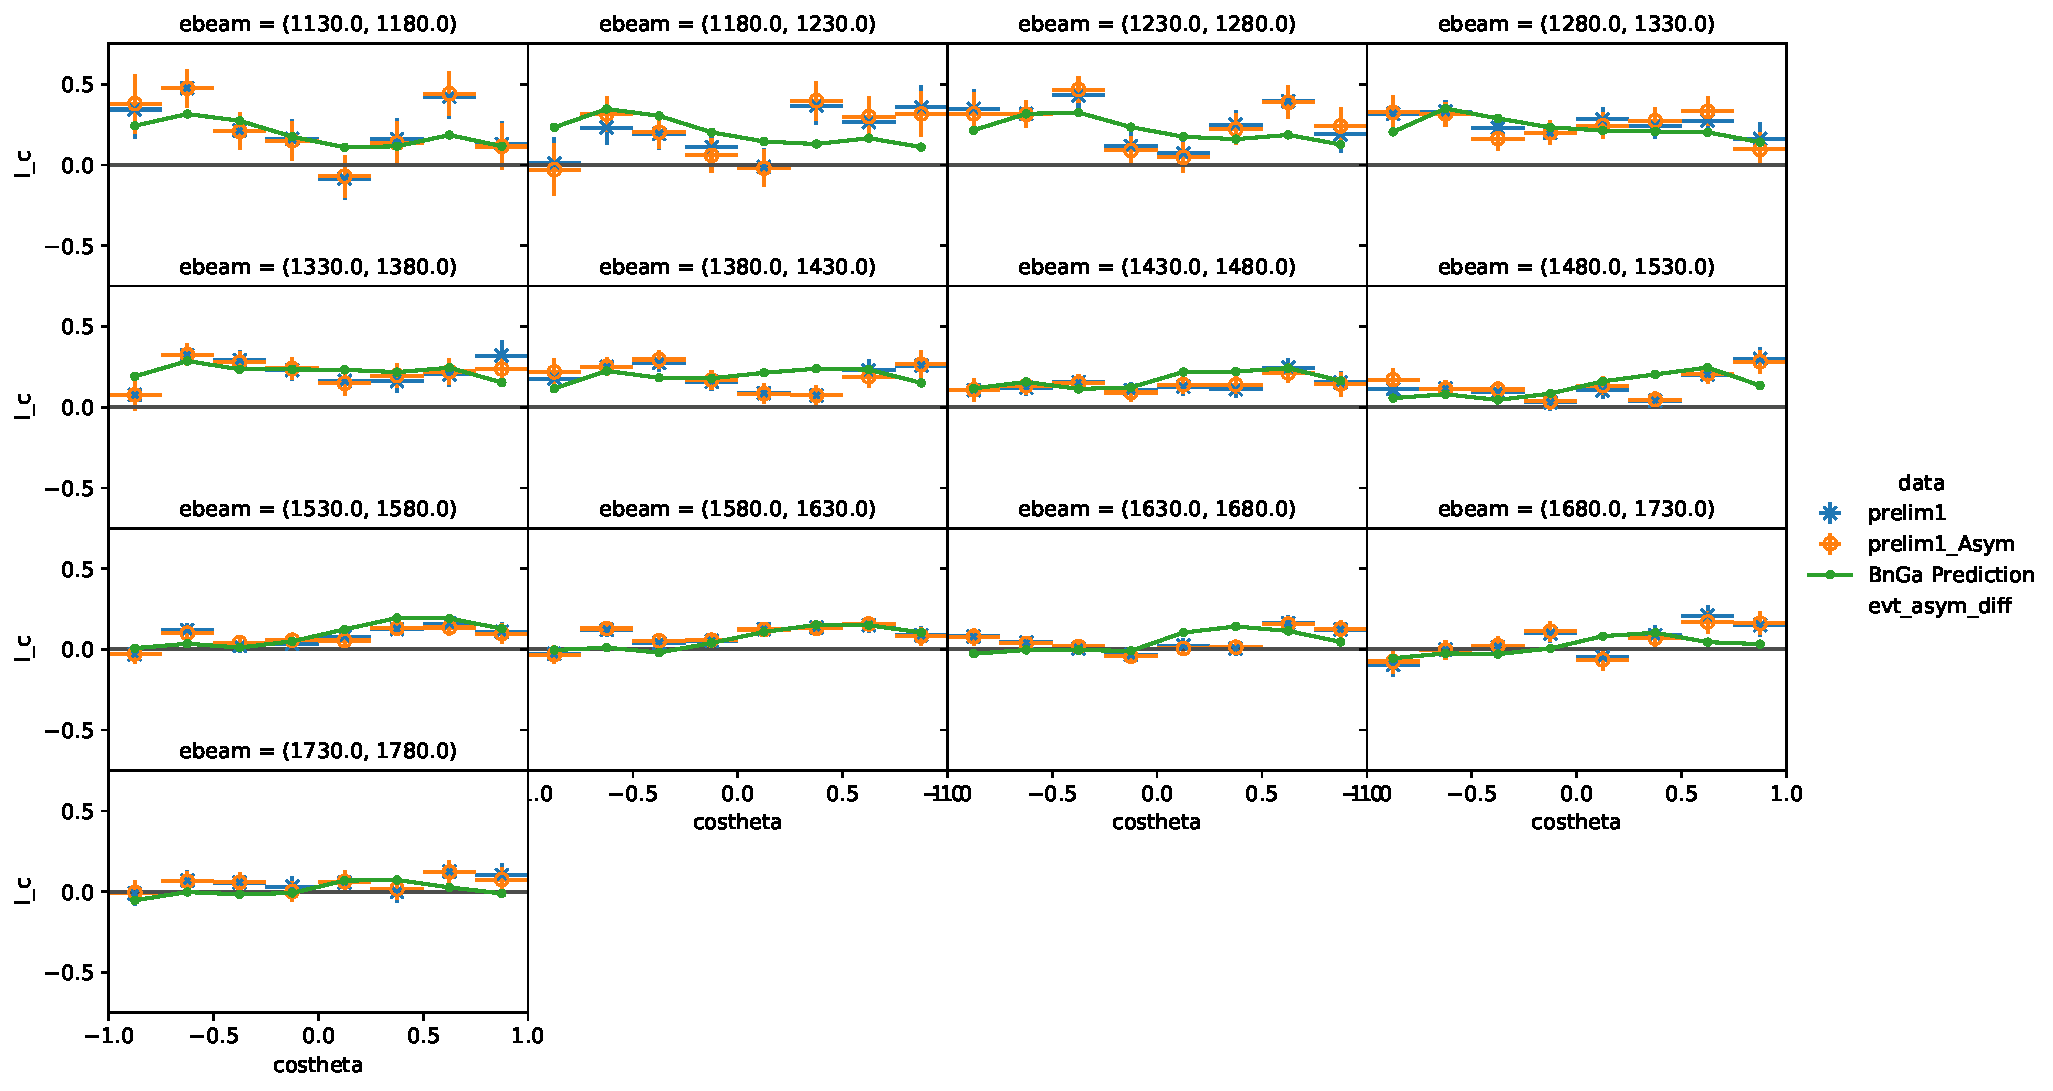
\includegraphics[width=\linewidth]{../../figs/hydrogen/asymmetry/2pi0_prelim.pdf}
\end{frame}

\begin{frame}{$\Sigma$ in $\gamma p \to p \eta'$}
	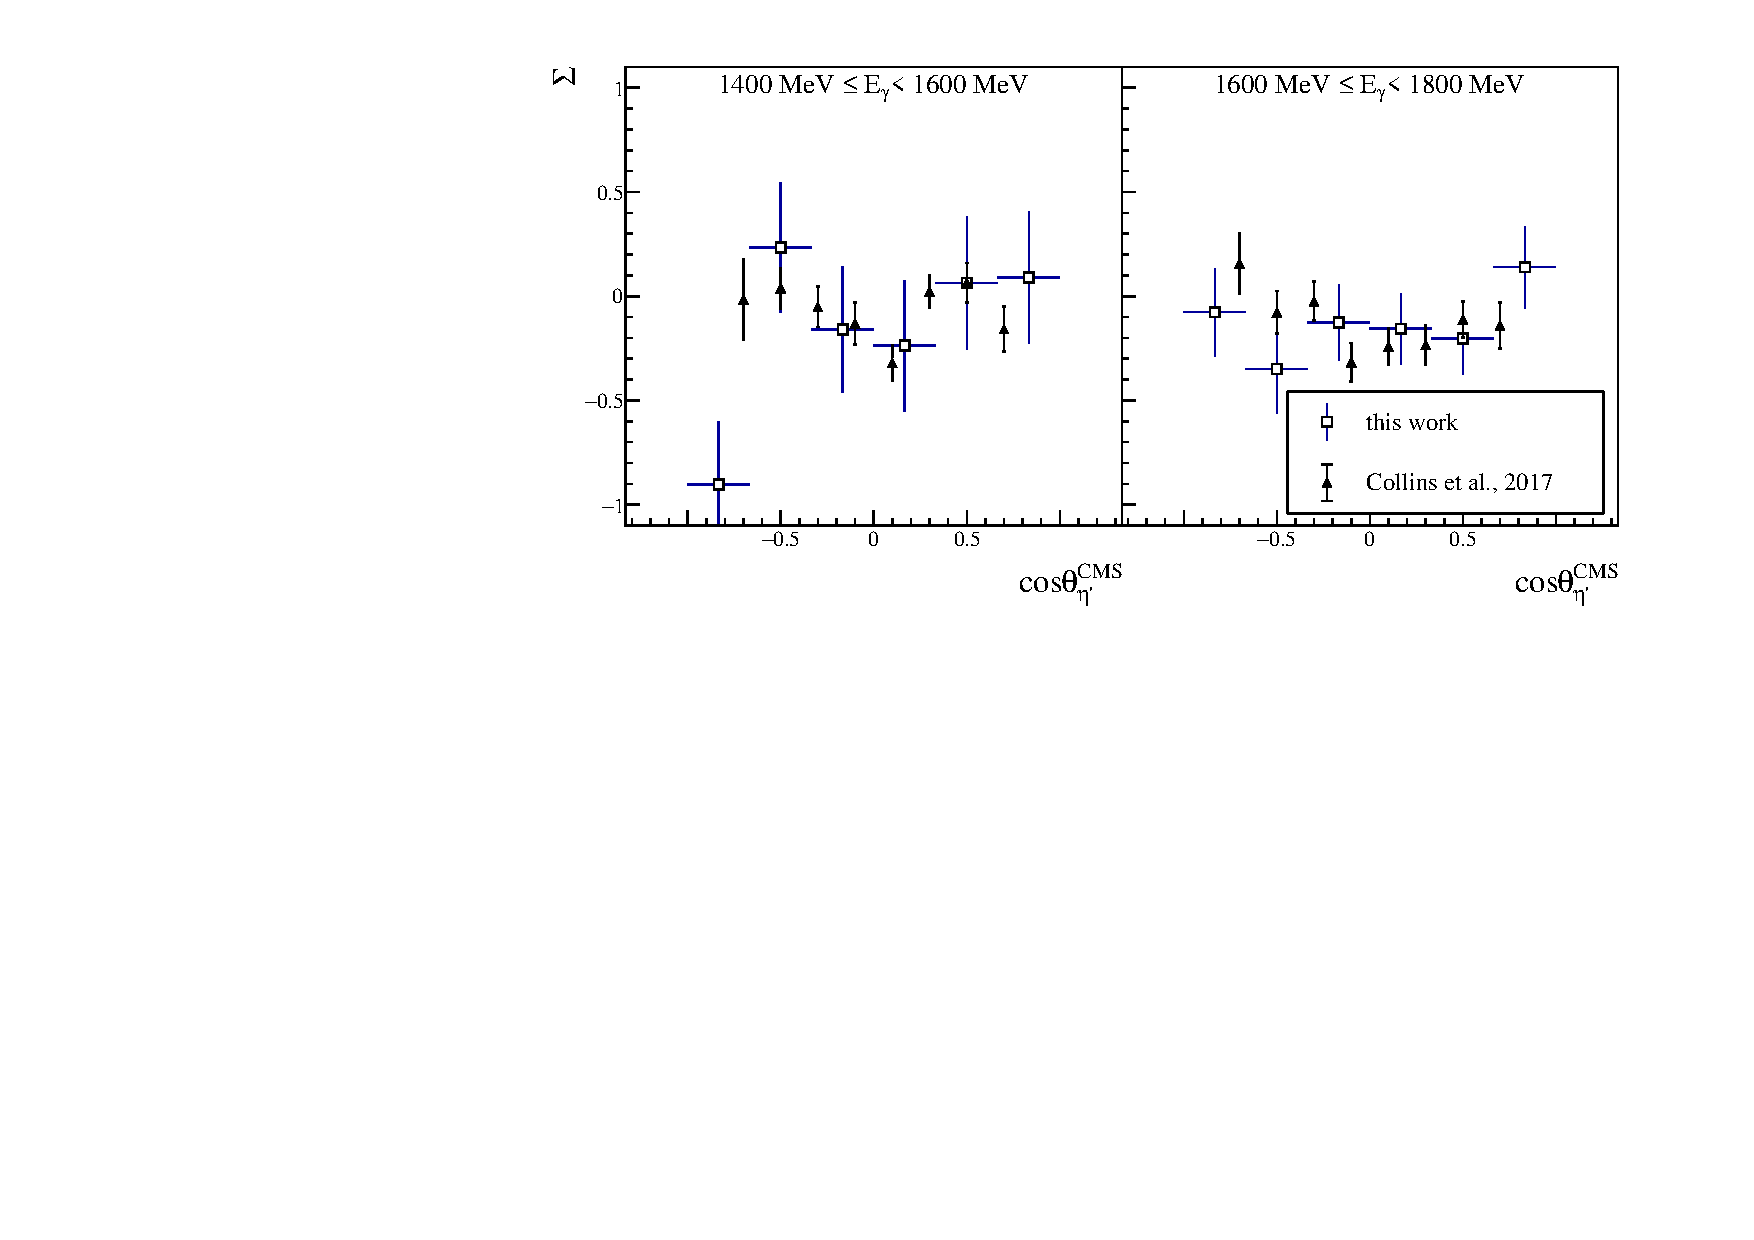
\includegraphics[width=\linewidth]{../../DPG2022/figs/sigma.pdf}
\end{frame}
\begin{frame}
\begin{tcolorbox}[colback=blue!5,colframe=\thecolor,title={To Do}]
	\begin{itemize}
		
		\item extract $\Sigma$ using unbinned maximum likelihood fit for $\eta'$
		\item apply \textsc{bayesian} approach 
		\item consider bkg contaminations in results of $\Sigma_{\eta'}$, study toy MC
		
	\end{itemize}
\end{tcolorbox}
\end{frame}




	
\end{document}
